\section{Study Design and Evaluation}
\label{sec:study-design-and-evaluation}

Fig.~\ref{fig:study-design} shows the main comparisons for the two prediction tasks.

\begin{figure}[t]
\centering
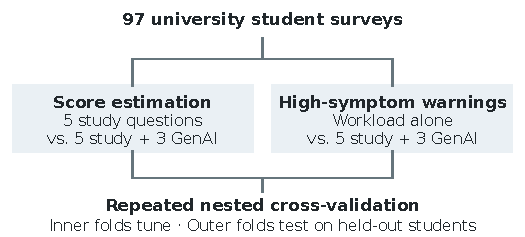
\includegraphics[width=\columnwidth]{figures/study-design.pdf}
\caption{Input sets for score estimation and high-symptom warnings. Numbers in parentheses give input counts.}
\label{fig:study-design}
\end{figure}

\subsection{Participants and Questionnaire}


We used convenience sampling to recruit Lebanese undergraduate and graduate students from multiple universities for an online cross-sectional survey. The survey link circulated primarily through WhatsApp among student contacts and their peers. We assessed eligibility using recruitment information and self-reported answers.

We analyzed all 97 survey submissions received from 4 to 18 October 2026. Of the respondents, 87 reported attending a university in Lebanon. Based on recruitment information, we identified the other 10 as Lebanese students studying abroad. After data collection, we revised the original location-based eligibility rule to include them.

The opening pages of the Google Forms survey explained the study and stated that participation was voluntary. Respondents indicated consent by choosing to continue. The form did not ask for names, contact information, or other direct identifiers. The study was not submitted for formal ethics review.

The questionnaire contained 20 questions on student background, study conditions, GenAI use, and intention to continue studying. It then presented the 23 core items of the English student version of the Burnout Assessment Tool (BAT-S)~\cite{schaufeli2020bat,batsenglishquestionnaire}. Short explanations clarified the word \emph{cynical} in BAT-S item Q33 and \emph{procrastinate} in the separate study-conditions item Q18.

\subsection{Outcomes and Data Preparation}

Responses to every BAT-S item used a scale from 1 (never) to 5 (always), with higher values indicating more frequent symptoms. For both scores, the calculation first averaged the items within each of the four dimensions. The four dimension means then contributed equally to the overall score.

The primary score used the 12 items marked as the short form in the English questionnaire. The secondary score used all 23 core items. Table~\ref{tab:bats-items} lists the survey question numbers for both scores. Each calculation required responses to all of its items, and both scores were complete for all 97 students.

\begin{table}[t]
\caption{Survey Items Used to Calculate the BAT-S Scores}
\label{tab:bats-items}
\centering
\footnotesize
\begin{tabular}{@{}lll@{}}
\hline
Dimension & Primary items & Core items \\
\hline
Exhaustion & Q21, Q23, Q24 & Q21--Q28 \\
Mental distance & Q29, Q31, Q33 & Q29--Q33 \\
Cognitive impairment & Q34, Q37, Q38 & Q34--Q38 \\
Emotional impairment & Q39, Q40, Q43 & Q39--Q43 \\
\hline
\end{tabular}
\end{table}

The warning task used the measured primary score to assign each student to one of two groups. A score of 4 or above defined the High group (17 students). Scores below 4 defined the Below-high group (80 students). Both groups describe symptom levels at the time of the survey.

Data preparation included checking the prepared data against the original export and recalculating the scores. One imported internet rating was corrected from the original answer, and one emotional-impairment mean was recalculated from its component items. When data were loaded for model fitting, three missing indicators of AI use for summarization were reconstructed from the original selections. The recoding completed the model inputs and left the prepared data file unchanged.

IBM SPSS Statistics 23 was used to summarize responses and scores and to calculate Cronbach's alpha for each dimension and for the 12-item and 23-item sets. Two-sided Spearman correlations examined 11 separate associations with the primary score without adjustment for multiple testing. A Pearson correlation was also calculated between AI dependence and the primary score.

\subsection{Input Sets and Score Prediction}

To test whether GenAI questions improved score prediction, we compared input sets using the same model family and evaluation splits within each comparison. Small A used five study-condition questions on perceived workload, sleep duration category, independent study-hours category, financial strain, and university support. Small B added three questions on GenAI use frequency, self-reported dependence on AI to complete academic work, and reliance on AI in place of independent thinking, for eight inputs.

Broad C used 13 inputs on background and study conditions (Q1--Q7 and Q14--Q19). It added eight questions to Small A, covering enrollment location, academic level, major, GPA range, electricity outages, internet quality, academic stress, and avoidance or procrastination.

Broad D added all six GenAI questions (Q8--Q13) to Broad C, covering frequency, use cases, dependence, reliance in place of independent thinking, verification of AI outputs, and concerns about being flagged for AI use. Q9 supplied separate yes-or-no inputs for concept explanations, writing, coding, summaries, and direct solutions, so 19 questions yielded 23 inputs before categorical encoding. All input sets excluded BAT-S responses and scores, submission timestamps, and the item on intention to continue studying.

The Small A and Small B comparison used linear regression, ridge regression, and a shallow random forest. The Broad C and Broad D comparison used ridge regression. The reference predictions were the mean and median measured scores in the training data.

Designated categorical inputs were encoded as separate indicators, with the first response category as the reference. For ridge regression, the encoded inputs were standardized using training data. The ridge penalty ranged from 0.01 to 1000 in tenfold steps. The regression forest used 200 trees, with candidate maximum depths of 2 and 3 and minimum leaf sizes of 5 and 10.

Score prediction used five repetitions of shuffled five-fold cross-validation. Each outer test fold held out one group of students for evaluation. Four inner folds within the remaining training data were used to select model settings by mean absolute error (MAE), the average absolute difference between predicted and measured scores. Predictions were clipped to the 1-to-5 scale during tuning and evaluation. MAE was calculated for the full sample and for students with measured scores of 4 or above.

Follow-up experiments gave more weight to errors for high scores. One comparison used a fixed equal-weight average of predictions from weighted ridge regression on Small B and support vector regression on Broad D.

\subsection{High-Symptom Warning Models}

The selected random forest classifier used Small B to predict the High label directly. The classifier used 100 trees, with candidate maximum depths of 2 and 3, minimum leaf sizes of 5 and 10, and relative training weights for the High group of 1, 2, and 4. The weights were rescaled within each fit to have a mean of 1.

The warning threshold determined when the classifier output triggered a warning. Candidate thresholds ranged from 0 to 1 in increments of 0.05. The separate cutoff of 4 applied to the measured BAT-S score and determined the student's group.

The augmentation procedure tested three quantities of synthetic profiles. It added zero, half as many, or as many profiles as there were real High students in the current training split. Fractional target counts were rounded up. Each synthetic profile was based on two High students from that split.

The distance between two students was the average of eight values. These were the six absolute differences in ordered responses, each divided by four, and two indicators of category mismatch. Eligible pairs had a distance of at most 0.35, and each ordered response differed by at most two points. The first student was selected at random from those with an eligible neighbor. The second was selected at random from up to three of the closest eligible neighbors.

The six ordered responses were interpolated using one shared fraction drawn uniformly from 0.2 to 0.8. Each resulting value was rounded probabilistically to a valid response value. The new profile inherited the first student's sleep and study-hours categories and was assigned a High label. To be accepted, a profile had to fall within 0.25 of the first student. Duplicates of real training profiles or previously accepted synthetic profiles in that split were rejected.

The comparison on real students included an eight-input forest tuned without augmentation. A logistic regression baseline using standardized perceived workload alone was added after the earlier model comparisons. It used \(L_2\) regularization with \(C=1\). The class weights and warning thresholds were selected from the same candidate values as for the forest.

Two fixed reference rules warned everyone or nobody. For the random reference, expected detections and false warnings were calculated for random selection of the same number of students as the forest warned in each outer test fold.

Earlier exploratory comparisons included support vector classifiers with a radial basis function kernel, using Small B or Broad D. These classifiers used real training data and tuned their settings and warning thresholds in the inner folds.

A separate historical fit used all 97 students. Its forest settings were depth 3, a minimum leaf size of 10, a relative High weight of 2, a warning threshold of 0.35, and zero synthetic training rows. The simulation applied this fitted model to 970 interpolated profiles. The profile labels were inherited from the students in the training data. The estimates for real students were obtained from the outer test folds described below.

\subsection{Warning Evaluation and Performance Measures}

The warning evaluation used five repetitions of stratified five-fold cross-validation to keep the proportion of High students similar across outer folds. For each outer test fold, four stratified inner folds within the training data were used to select model settings, class weight, augmentation ratio, and warning threshold where applicable.

Selection used the pooled inner-fold \(F_2\) score, which gives greater weight to recall than precision. Ties favored higher precision, higher recall, a higher warning threshold, and then a smaller augmentation ratio where applicable.

For the forest, the sleep and study-hours categories were encoded and the resulting columns were standardized using the corresponding training data. Synthetic profiles for each fit were generated from the same training split. Only held-out real students contributed predictions to the outer evaluation. The reproduced ridge and warning evaluations used scikit-learn version 1.9.1. The other model comparisons are reported from their analysis records.

The held-out predictions were pooled within each repetition, so each student contributed once per repetition. Recall is the share of High students detected, and precision is the share of warnings issued to High students. Balanced accuracy averages the correct classification rates of the two groups. Average precision and the area under the receiver operating characteristic curve summarized ranking across thresholds. Each measure was averaged across the five repetitions.

The chance comparison shuffled the student labels 199 times while preserving the overall class counts. Each shuffle assigned one label per student across all repetitions. For each shuffle, the stratified splits were rebuilt and the selected forest procedure was repeated, including the inner selection and training-only generation of synthetic profiles. The comparison used mean balanced accuracy, as specified in the validation plan. The one-sided permutation \(p\)-value was \((b+1)/200\), where \(b\) counts shuffled runs that reached or exceeded the observed value~\cite{phipson2010permutation}.

Uncertainty was estimated from 2,000 bootstrap samples. Students were resampled with replacement within each outcome group. Each sampled student carried all five held-out predictions, and the models were compared using the same resamples. The 95\% percentile intervals describe variation conditional on the observed class counts and fitted predictions.
